\documentclass[tikz, border=5pt]{standalone}

\begin{document}
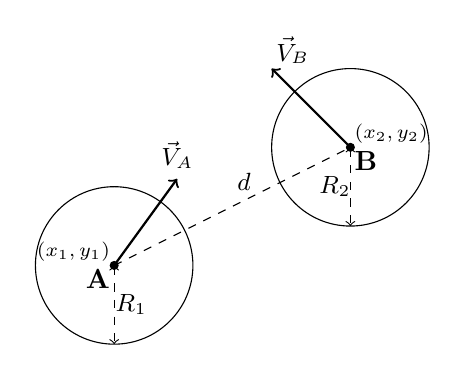
\begin{tikzpicture}

    %% Collision diagram

    % Mass A
    \coordinate (A) at (0,0);
    \draw[fill] (A) circle (0.05) node[below left=-2] {\( \mathbf A \)};
    \node[above left=-2] at (A) {\scriptsize \( (x_1, y_1) \)};
    \draw[->, thick] (A) -- ++(0.8,1.1) node[above] {\small \( \vec{V}_A \)};
    \draw (A) circle (1);
    \draw[<->, dashed] (A) -- ++(0,-1) node[midway, right=-3] {\small \( R_1 \)};

    % Mass B
    \coordinate (B) at (3,1.5);
    \draw[fill] (B) circle (0.05) node[below right=-2] {\( \mathbf B \)};
    \node[above right=-2] at (B) {\scriptsize \( (x_2, y_2) \)};
    \draw[->, thick] (B) -- ++(-1,1) node[above right=-2] {\small \( \vec{V}_B \)};
    \draw (B) circle (1);
    \draw[<->, dashed] (B) -- ++(0,-1) node[midway, left=-3.5] {\small \( R_2 \)};

    % Line of separation
    \draw[dashed] (A) -- (B) node[pos=0.55, above] {\small \( d \)};

\end{tikzpicture}
\end{document}
